\documentclass[PhD]{PHlab-thesis}

\addbibresource{thesis.bib}

\newcommand*\Department中文{資訊工程學系}
\newcommand*\Department英文{Department of Computer Science and Information Engineering}

\newcommand*\ThesisTitle中文{利用GPU加速mtDNA與nDNA序列在Smith-Waterman with affine gap Algorithm上的比對\退{1}}
\newcommand*\ThesisTitle英文{Accelerating mtDNA and nDNA Sequence Alignment Using the Smith-Waterman with affine gap Algorithm on GPU}


\newcommand*\Student中文{楊祐昇}
\newcommand*\Student英文{You-Sheng Yang}

\newcommand*\Advisor中文{賀保羅}
\newcommand*\Advisor英文{Paul Horton}

%% 果有共同指導老師可以用:
%% \newcommand*\CoAdvisorA中文{}
%% \newcommand*\CoAdvisorA英文{}
%% \newcommand*\CoAdvisorB中文{}
%% \newcommand*\CoAdvisorB英文{}
\usepackage{subcaption}
\usepackage{algorithm}
\usepackage{algpseudocode}
\usepackage[table]{xcolor}


\newcommand*\YearMonth英文{June, 2025}
\newcommand*\YearMonth中文{114年6月}

\pagestyle{fancy}% Use fancyhdr
\begin{document}


\newcommand*\Keywords英文{Large-Scale Genomic Sequence Alignment, GPU acceleration, local alignment with affine gap, Smith-Waterman Algorithm, CUDA}
\newcommand*\Abstract英文{%
Sequence alignment plays a critical role in bioinformatics and molecular biology. It is widely used in various analyses such as gene function prediction, evolutionary studies, and disease research. However, these methods generally exhibit quadratic time complexity, leading to a rapid increase in computational resources and time costs when handling large-scale genomic data, thus becoming a major bottleneck in biological data analysis.

The primary objective of this study is to design and implement a high performance acceleration method for local alignment between human mitochondrial DNA (mtDNA) and nuclear genome (nDNA) sequences. Our approach is based on the Compute Unified Device Architecture (CUDA) platform and incorporates the Smith-Waterman algorithm with an affine gap penalty model. By optimizing GPU memory allocation, accelerating memory access, and modifying the core algorithm—drawing upon techniques from \cite{CUDAlign}—we significantly enhance both the efficiency and scalability of local alignment. Furthermore, through experimentation, we identified the optimal number of threads for different GPU architectures, ultimately developing a practical alignment tool for large-scale genomic sequences such as mtDNA and nDNA.

Experimental results demonstrate that the developed tool achieves significant speedup and provides graphical analysis capabilities, enabling users to perform customized analyses according to their specific needs. The tool has been made publicly available on the GitHub platform and can be freely downloaded and used via the following link:\hyperlink{https://github.com/YYS13/LargeScaleSW}{https://github.com/YYS13/LargeScaleSW}.}


\newcommand*\Keywords中文{大型基因體序列比對、GPU加速、帶有仿射間隙懲罰的區域比對、Smith-Waterman演算法、CUDA}
\newcommand*\Abstract中文{%
基因序列比對在生物資訊學與分子生物學中扮演非常重要的角色,它可以被用在基因功能預測、物種演化分析、疾病研究等各種分析上,然而這些方法通常具有平方級的時間複雜度,導致在面對大規模基因體資料時,所需的計算資源及時間成本急遽增加,成為分析上的一大瓶頸。

本篇論文研究的主要目標,旨在針對人類粒線體(mtDNA)與核基因體(nDNA)序列的局部比對問題,設計並實作一套高效能的加速方法,我們基於 Compute Unified Device Architecture (CUDA) 平台,根據 Smith-Waterman 這個演算法並加入仿射間隙懲罰(affine gap penalty)模型,透過優化\cite{CUDAlign}在 GPU 記憶體空間分配,加速 GPU 存取記憶體速度以及修改其演算法,進一步提升了局部比對的整體效率與可擴展性,除此之外我們透過實驗找出在不同的 GPU 上最適合的 threads 數量,實作出適用於粒線體與核基因體等此類大型基因序列的比對工具。

實驗結果證實該工具不僅實現了顯著的加速效果,並提供圖表化的分析,讓使用者可以根據自身需求進行分析,本研究成果已開放於 GitHub 平台,使用者可透過以下連結取得並自由下載使用本工具:\hyperlink{https://github.com/YYS13/LargeScaleSW}{https://github.com/YYS13/LargeScaleSW}
}

\newcommand*\Acknowledgements{%
首先我要感謝我的指導教授賀保羅教授,感謝教授這兩年的細心指導與提點,透過教授的課程與會議上的教學,讓我對生醫資訊這個領域有更多的認識,也因此有這篇碩士論文的誕生。另外我要感謝已經畢業的學姊昱伶,在找教授時給我許多的幫助。還有我實驗室同學書堯、祈翰、驊軒、煜醴、 尊緯、晴文、宜靜以及考研時的戰友秉為,不論在學業上或是休閒娛樂都有你們陪伴、互相成長,讓我可以順利度過碩士生活。最後要感謝我的家人和女朋友,感謝有他們的陪伴讓我在這條路上不孤單。感謝這些貴人的出現,我才可以完成我的碩士論文。
}



\newcommand*\SelectFontsize[2]{\fontsize{#1}{#1}\selectfont\mdseries#2\par}
\newcommand*\SelectFontsizeBF[2]{\fontsize{#1}{#1}\selectfont\bfseries#2\par}
\newcommand*\SignatureRule[1][6]{\rule{#1cm}{0.3mm}}
\newcommand*\AddToContents[1]{\newpage\phantomsection\addcontentsline{toc}{chapter}{#1}}

\doublespace
\pagenumbering{gobble}
\renewcommand{\thefootnote}{\fnsymbol{footnote}}


\begin{center}
\vspace{2cm}
\SelectFontsizeBF{24}{%
\University中文\Department中文\\
\學位 論文}

\vfill
\SelectFontsizeBF{24}{\ThesisTitle中文}
\ifdefined\ThesisNote中文
\SelectFontsize{22}{\textit{\ThesisNote中文}}
\fi

\vspace{5mm}
\SelectFontsizeBF{22}{\ThesisTitle英文}
\ifdefined\ThesisNote英文
\SelectFontsize{20}{\textit{\ThesisNote英文}}
\fi

\vfill

\begin{minipage}{\linewidth}
{\setlength\tabcolsep{0pt}
%
\begin{tabular}{ Wr{5em} Wl{6em} Wr{5em} wl{7em} }
研究生:   & ~~\Student中文  &      Student: & ~~\Student英文\\
指導老師: & ~~\Advisor中文  &      Advisor: & ~~\Advisor英文\\
\ifdefined\CoAdvisorA中文
共同指導: & ~~\CoAdvisorA中文 &   Co-Advisor: & ~~\CoAdvisorA英文\\
\fi
\ifdefined\CoAdvisorB中文
         & ~~\CoAdvisorB中文 &   Co-Advisor: & ~~\CoAdvisorB英文\\
\fi
\end{tabular}
}
\end{minipage}

\vfill
\SelectFontsize{18}{%
National Cheng Kung University,\\
Tainan, Taiwan, R.O.C.\\
Thesis for \ifdef\PhD{Master of Science}{Doctor of Philosophy} Degree\\
\YearMonth英文}

\vfill
\SelectFontsize{20}{中華民國\YearMonth中文}
\end{center}



\ifdefined\optCommittee
\newpage
\begin{center}
\vspace{1cm}
\SelectFontsizeBF{24}{%
\University中文\Department中文\\
\學位 論文}
\vfill
\SelectFontsizeBF{20}{\ThesisTitle中文}
\end{center}

\vfill
\SelectFontsize{20}{%
\noindent 研究生:\Student中文\\
本論文業經審查及口試合格特此證明}


\begin{center}
\SelectFontsize{18pt}{論文考試委員}
\vfill
\SignatureRule \hspace*{1cm} \SignatureRule
\vfill

\SignatureRule \hspace*{1cm} \SignatureRule
\vfill

指導教授:\SignatureRule[8]
\vfill
  所長:\SignatureRule[8]

\vfill
\SelectFontsize{18}{中華民國 \hspace{2em} 年 \hspace{2em} 月 \hspace{2em} 日}
\end{center}


\newpage
\begin{center}
\vspace{1cm}
\SelectFontsize{18}{\University英文, \Department英文}
\SelectFontsize{19}{\ifdef\PhD{Ph.D.}{Master's} Degree Thesis}

\vfill
\SelectFontsizeBF{20}{\ThesisTitle英文}
\end{center}

\vfill
\SelectFontsize{18}{Student: \Student英文}

\SelectFontsize{18}{%
A thesis submitted to the graduate division in partial fulfillment of the requirement for the degree of
\ifdef\PhD{Master of Science}{Doctor of \mbox{Philosophy}}.
}

\vfill
\begin{center}
\SelectFontsize{18}{Approved by}

\vfill
\SignatureRule \hspace*{1cm} \SignatureRule

\vfill
\SignatureRule \hspace*{1cm} \SignatureRule

\vfill
Advisor: \SignatureRule[8]

\vfill
Chairman: \SignatureRule[8]

\vfill
\SelectFontsize{18}{\YearMonth英文}
\vspace*{20pt}
\end{center}
\fi% optCommittee


\AddToContents{中文摘要}
\setcounter{page}{1}
\pagenumbering{roman}


\begin{center}
\SelectFontsizeBF{24}{\ThesisTitle中文}

\vspace{4mm}
\SelectFontsize{18}{\Student中文\footnote[1]{學生} ~ \Advisor中文\footnote[2]{指導教授}}

\vspace{5mm}
\SelectFontsize{20}{國立成功大學\Department中文}

\vspace{12mm}
\makebox[2.7cm][c]{\SelectFontsizeBF{22}{摘要}}
\end{center}

\vspace{4mm}
\SelectFontsize{16}{\Abstract中文}

\vspace{4mm}
\begin{flushleft}
\SelectFontsize{16}{\textbf{關鍵詞:} \Keywords中文}
\end{flushleft}



\AddToContents{Abstract}
\begin{center}
\SelectFontsizeBF{22}{\ThesisTitle英文}

\vspace{4mm}
\SelectFontsize{18}{\Student英文\footnote[1]{Student} ~ \Advisor英文\footnote[2]{Advisor}}

\vspace{4mm}
\SelectFontsize{16}{\Department英文, National Cheng Kung University}

\vspace{12mm}
\SelectFontsizeBF{20}{Abstract}
\end{center}

\vspace{4mm}
\SelectFontsize{14}{\Abstract英文}

\vspace{4mm}
\begin{flushleft}
\SelectFontsize{16}{\textbf{Keywords:} \Keywords英文}
\end{flushleft}



\AddToContents{誌謝}
\begin{center}\SelectFontsizeBF{24}{誌謝}\end{center}

\vspace{4mm}
\Acknowledgements



\renewcommand{\contentsname}{CONTENTS}
\AddToContents{Contents}
\tableofcontents


\AddToContents{List of Tables}
\listoftables


\AddToContents{List of Figures}
\listoffigures
% 封面頁, 口委中英文簽名單, 誌謝, 中英文摘要, 論文目錄, 圖表目錄


%────────────────────  List of Symbols  ────────────────────
\renewcommand\nomgroup[1]{%
  \item[\bfseries
  \ifstrequal{#1}{A}{General}{%
  }]}

\nomenclature[A]{GPU}{Graphics Processing Unit}
\nomenclature[A]{CUDA}{Compute Unified Device Architecture}
\nomenclature[A]{GPGPU}{General-Purpose computing on Graphics Processing Units}

\printnomenclature[5cm]

\newpage
\setcounter{page}{1}
\pagenumbering{arabic}



\chapter{Introduction}
\section{Background and Motivation}
In recent years, the rapid development of Next-Generation Sequencing (NGS) has significantly reduced the cost of DNA sequencing. As a result, researchers can now obtain high-sensitivity and high-resolution data more efficiently \cite{NGS1}\cite{NGS2}. Moreover, read lengths can be flexibly adjusted according to research needs. These advancements have enabled researchers to more accurately analyze variations, similarities, and structural features among gene sequences, making NGS a cornerstone of modern genomics and precision medicine.

Among the various analytical methods, local alignment algorithm play a crucial role. it is widely used in fields such as bioinformatics, medical diagnostics, and evolutionary analysis. Among these algorithms, the Smith-Waterman algorithm is known for its high precision. It uses dynamic programming to identify the optimal local alignment between two sequences. However, both its time and space complexities are $O(mn)$, where $m$ and $n$ denote the lengths of the two sequences being aligned. This high computational demand poses a significant challenge for researchers, especially when dealing with large-scale genomic alignments.

In the human genome, mitochondrial DNA (mtDNA) is a small circular double-stranded DNA molecule located within the mitochondria, with a length of approximately 16,569 base pairs. It primarily encodes proteins involved in cellular energy metabolism. In contrast, nuclear DNA (nDNA), stored within the cell nucleus, is a linear molecule encompassing the vast majority of human genetic information, with a total length reaching several billion base pairs. During the course of evolution, fragments of mtDNA can become integrated into the nuclear genome through insertion events, forming what are known as nuclear mitochondrial DNA segments (NUMTs). However, due to molecular events such as mutations and genomic rearrangements, NUMTs often diverge significantly from their original mtDNA sequences.

According to \cite{NUMTs1}, a comprehensive analysis of over 66,000 human genomes revealed that NUMTs are widely distributed across the nuclear genome, indicating that they represent a common and biologically significant phenomenon. Consequently, performing high-resolution local sequence alignment between mtDNA and nDNA is crucial not only for accurately identifying the locations and structures of NUMTs, but also for elucidating their roles in evolutionary processes and potential functional transformations. Furthermore, such alignments have important applications in disease-related research and the detection of pathogenic mutations.

However, as previously noted, the Smith-Waterman algorithm, while offering optimal alignment accuracy, has a computational complexity of $O(mn)$. When aligning sequences with vastly different lengths, such as mtDNA and nDNA, even a single comparison using one set of alignment parameters may take several hours to days. Additionally, due to the size of the nDNA, memory consumption can reach several hundred terabytes. When multiple parameter sets are required for comparative or sensitivity analyses, the computational and memory demands become a major bottleneck, posing significant challenges to large-scale and high-precision genomic alignment studies.

With the advancement of parallel computing technologies, Graphics Processing Units (GPUs) have recently been widely recognized as a high-performance and relatively low-cost acceleration platform. Furthermore, with the introduction of CUDA (Compute Unified Device Architecture) \cite{CUDA1, CUDA2}, developers can write programs directly in high-level languages such as C/C++ to execute on NVIDIA GPUs, significantly lowering the barrier to parallel programming. Numerous CUDA-based approaches have been proposed to accelerate sequence alignment algorithms \cite{CUDA4, CUDA5}, but most of these methods are limited to sequences of equal length and impose strict constraints on sequence size, which makes them impractical for real-world sequence alignment tasks.

To the best of our knowledge, there is currently no available CUDA-based tool that effectively handles the alignment of large genomic sequences with significant length disparities, such as mitochondrial DNA (mtDNA) and nuclear DNA (nDNA), using the Smith-Waterman algorithm with an affine gap penalty model. To address this limitation, we propose the development of a high-performance and practical alignment tool that leverages CUDA's parallel computing capabilities in conjunction with the precise Smith-Waterman dynamic programming algorithm, incorporating the affine gap penalty model. This tool aims to support the alignment of highly divergent sequence lengths, significantly reducing analysis time while enhancing overall alignment efficiency and applicability.

\section{Smith-Waterman Algorithm}
The Smith–Waterman algorithm was first proposed by Smith and Waterman in 1981 \cite{Smith-Waterman}. It is a local alignment method based on dynamic programming that aims to identify the most similar region between two sequences. By computing a score matrix and performing traceback, it obtains the optimal local alignment.
In 1982, Gotoh introduced the affine gap penalty model \cite{Affine-Gap}, pointing out that the traditional linear gap penalty does not accurately reflect real biological sequences—biologically, a continuous gap carries more significance than an isolated single gap. Consequently, opening a gap (gap opening) should incur a larger penalty than extending an existing gap (gap extension). Gotoh’s approach maintains computational efficiency while improving alignment accuracy.
The Smith–Waterman algorithm with an affine gap penalty as follows:

\[
\begin{alignedat}{2}
E_{i,j} &= \max \left\{ 
    \begin{array}{l}
        H_{i-1,j} - G_{\text{open}} \\
        E_{i-1,j} - G_{\text{extend}}
    \end{array} \right. \\
    \\
F_{i,j} &= \max \left\{
    \begin{array}{l}
        H_{i,j-1} - G_{\text{open}} \\
        F_{i,j-1} - G_{\text{extend}}
    \end{array} \right. \\
    \\
H_{i,j} &= \max \left\{
    \begin{array}{l}
        0 \\
        H_{i-1,j-1} + W(S_0[i], S_1[j]) \\
        E_{i,j} \\
        F_{i,j}
    \end{array} \right.
\end{alignedat}
\]

Let $S_{0}$ be the query sequence and $S_{1}$ the target sequence;  
in this study they correspond to the mtDNA and a human chromosome,  
with lengths $m$ and $n$, respectively.The dynamic-programming matrices $\mathbf{E}$, $\mathbf{F}$, and $\mathbf{H}$  
store the optimal local alignment scores under different states for every cell and are each of size $(m+1)\times(n+1)$:
\begin{itemize}
  \item $E_{i,j}$ — best score at cell $(i,j)$ when the alignment ends with a
        \emph{vertical gap} (deletion);
  \item $F_{i,j}$ — best score at cell $(i,j)$ when the alignment ends with a
        \emph{horizontal gap} (insertion);
  \item $H_{i,j}$ — best score at cell $(i,j)$ when the alignment ends with a
        \emph{match or mismatch}.
\end{itemize}

\noindent
Consequently, the Smith--Waterman algorithm with an affine gap penalty requires both time and space complexities of $O(mn)$.Figure\ref{fig:Score Matrix} and Figure\ref{fig:Alignment Result} shows the alignment result and the corresponding score matrix for two sequences using the parameters: $Match = 3$, $Mismatch = -1$, $OpenGap = -5$, and $ExtendGap = -1$.

\begin{figure}[h]
    \centering
    \begin{subfigure}{0.9\textwidth}
        \centering
        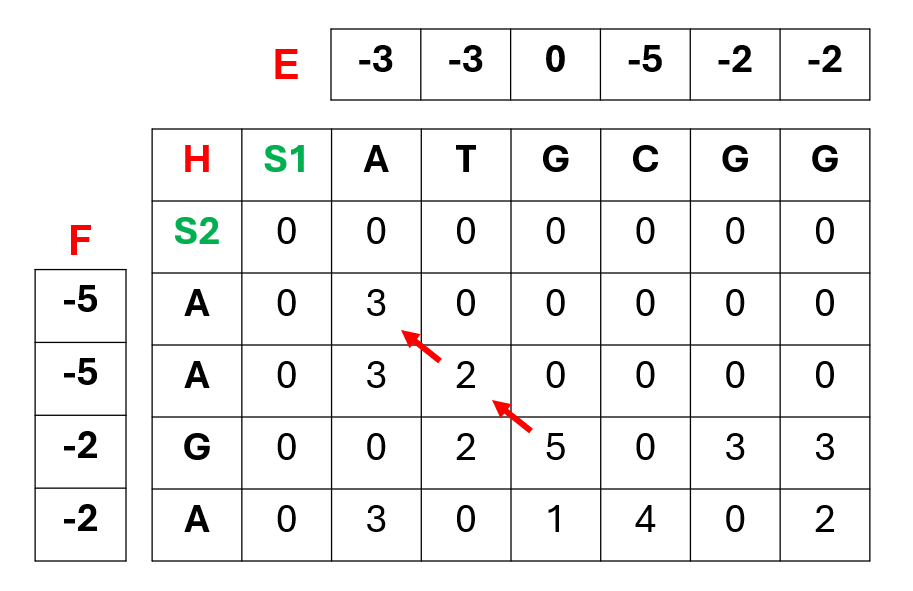
\includegraphics[width=\textwidth]{figures/scoreMatrix.png}
        \caption{Score Matrix}
        \label{fig:Score Matrix}
    \end{subfigure}

    \vspace{0.5cm}

    \begin{subfigure}{0.9\textwidth}
        \centering
        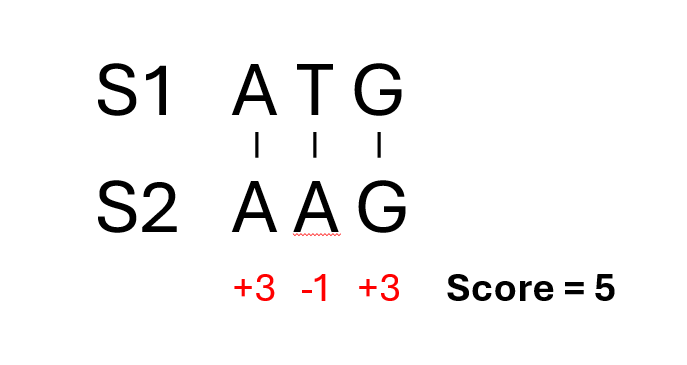
\includegraphics[height=5cm]{figures/alignmentResult.png}
        \caption{Alignment Result}
        \label{fig:Alignment Result}
    \end{subfigure}

    \caption{Score matrix and alignment result of two sequences}
    \label{fig:ScoreMatrixAlignmentResult}
\end{figure}



\clearpage
\section{CUDA architecture}

CUDA (Compute Unified Device Architecture) is a parallel-programming software platform introduced by Nvidia\cite{CUDA1, CUDA2}. Its purpose is to let developers tap into Nvidia GPUs for a wide range of parallel computations through a consistent architecture while writing in high-level languages such as C, C++, and Fortran. These advantages have made CUDA the most widely adopted development platform in the GPGPU (General-Purpose computing on Graphics Processing Units) domain.

In CUDA, program execution can be managed across three hierarchical levels, namely \textbf{Grid}, \textbf{Block}, and \textbf{Thread} arranged from top to bottom. A Grid consists of multiple Blocks, and each Block is composed of multiple Threads. A Thread represents the most fundamental unit of execution, responsible for performing actual computational tasks. The Grid defines the overall computational space available during a single kernel launch. To initiate computation, the syntax \texttt{\textbf{kernel<<<B, T>>>(...)}} is used, where $B$ and $T$ denote the number of Blocks and Threads, respectively. The term kernel refers to functions written by developers that can be executed on the GPU.

Moreover, memory access management is often a critical factor affecting the performance of CUDA programs. In CUDA, the memory hierarchy is primarily divided into five levels: \textbf{Registers}, \textbf{Shared Memory}, \textbf{Constant Memory}, \textbf{Texture Memory}, and \textbf{Global Memory}. There is an inverse relationship between access speed and memory capacity, with access speed decreasing and capacity increasing from left to right across these levels. Each memory type has its own access rules and limitations, as detailed below:

\begin{itemize}
  \item \textbf{Registers}: Read-Write, used exclusively by a single thread (allocated based on the number of threads within a single block).
  \item \textbf{Shared Memory}: Read-Write, shared among all threads within a block.
  \item \textbf{Constant Memory}: Read-only, accessible by all threads.
  \item \textbf{Texture Memory}: Read-only, accessible by all threads.
  \item \textbf{Global Memory}: Read-Write, accessible by all threads.
\end{itemize}

Developers must design efficient GPGPU algorithms based on the above architectural constraints. Figure \ref{fig:CUDA Architecture} shows the schematic diagram of the CUDA architecture described above.
\begin{figure}[ht]
    \centering
    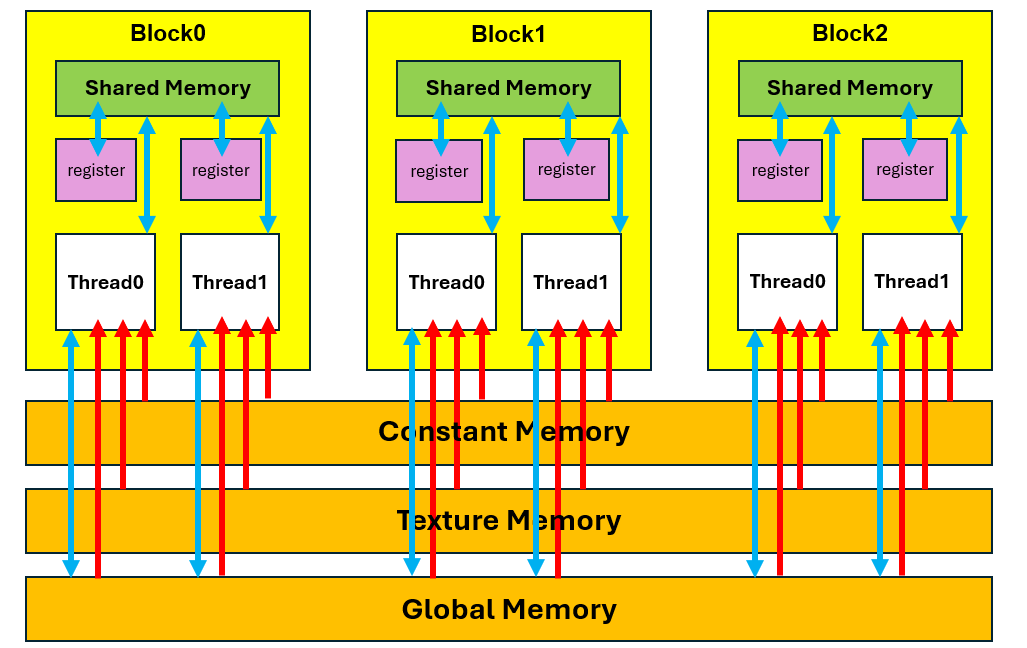
\includegraphics[width = 1\textwidth]{figures/CUDA_Architecture.png}
    \caption{CUDA Architecture}
    \label{fig:CUDA Architecture}
\end{figure}

\chapter{Related Work}
In prior research, many efforts have been devoted to improving the performance of sequence alignment algorithms on GPUs. Nauman Ahmed et al. \cite{CUDA3} proposed a GPU-accelerated alignment library called GASAL, which significantly speeds up performance—up to 200 times faster—by moving the data packing (sequence compression) process from the CPU to the GPU, compared to the original NVBIO implementation. Kailash W. Kalare et al. \cite{CUDA6} adopted an anti-diagonal parallelization strategy, dividing the task matrix into outer and inter diagonals. The outer diagonal corresponds to block-level parallelism in CUDA, while the inter diagonal maps to thread-level parallelism. All blocks on the same anti-diagonal can execute their internal thread computations simultaneously, thereby enhancing performance. Edans Flavius de O. Sandes et al. \cite{CUDAlign} introduced the Cell Delegation technique, combining it with anti-diagonal parallelization to significantly increase the number of threads executable per time unit. They applied this approach to large-scale genomic sequence alignment, overcoming previous research limitations that mainly focused on short sequence alignment and dramatically increasing the length and scale of alignable sequences.

However, these studies are mostly applied to short sequences of equal length or encounter challenges such as inefficient memory access and difficulties in identifying alignment regions in large-scale genomic comparisons. Furthermore, there is still a lack of GPU-accelerated alignment tools specifically designed for sequences with significantly different lengths (e.g., mtDNA vs. nDNA). To address this, we integrate the strengths of the aforementioned studies and propose an improved CUDA-based implementation of the Smith-Waterman algorithm with affine gap penalties. This tool supports local alignment and mapping between large genomic sequences with highly disparate lengths and enhances GPU memory access efficiency. The detailed methodology will be presented in the next chapter.











\chapter{Methods}
\section{Anti-Diagonal Strategy and Data Dependency}
The Anti-Diagonal strategy is a commonly used method in GPU-accelerated research on sequence alignment algorithms. Due to the data dependency inherent in these algorithms, the computation of any given matrix cell requires prior access to its left, upper-left, and upper neighboring cells. Therefore, cells located on the same anti-diagonal do not have data dependencies among each other. As a result, the main anti-diagonal of the matrix offers the highest degree of parallelism. In the case of the Smith-Waterman algorithm with affine gap penalties used in this study, the data dependency pattern is as follows:

\begin{itemize}
    \item $H_{i,j}$ depends on $H_{i-1,j-1}$, $H_{i-1,j}$, $H_{i,j-1}$, $E_{i-1,j}$ and $F_{i,j-1}$ 
    \item $E_{i,j}$ depends on $H_{i-1,j}$ and $E_{i-1,j}$.
    \item $F_{i,j}$ depends on $H_{i,j-1}$ and $F_{i,j-1}$.
\end{itemize}

Figure~\ref{fig:Anti-Diagonal and Dependency diagram} illustrates the dependency pattern of cells along the anti-diagonal in the algorithm used in this study.For any cell $H_{i,j}$on the same anti-diagonal where $i+j=k$, its value depends on the previous anti-diagonal where $i + j = k - 2$, as well as the values from the same anti-diagonal in the $E$ and $F$ matrices. The values in the same anti-diagonal of the $E$ and $F$matrices, in turn, are derived from the previous anti-diagonal where $i + j = k - 1$.Therefore, cells with the same color are independent of each other and can be computed in parallel. Furthermore, by adopting the anti-diagonal strategy, cells on the same diagonal do not overlap in accessing the $E$ and $F$ matrices. As a result, the $E$ and $F$ matrices can be compressed into one-dimensional arrays, significantly reducing memory usage and improving memory access efficiency in GPU. The optimization details regarding GPU memory access efficiency will be further discussed in the next section.
\vspace{0.5cm}
\begin{figure}[ht]
    \centering
    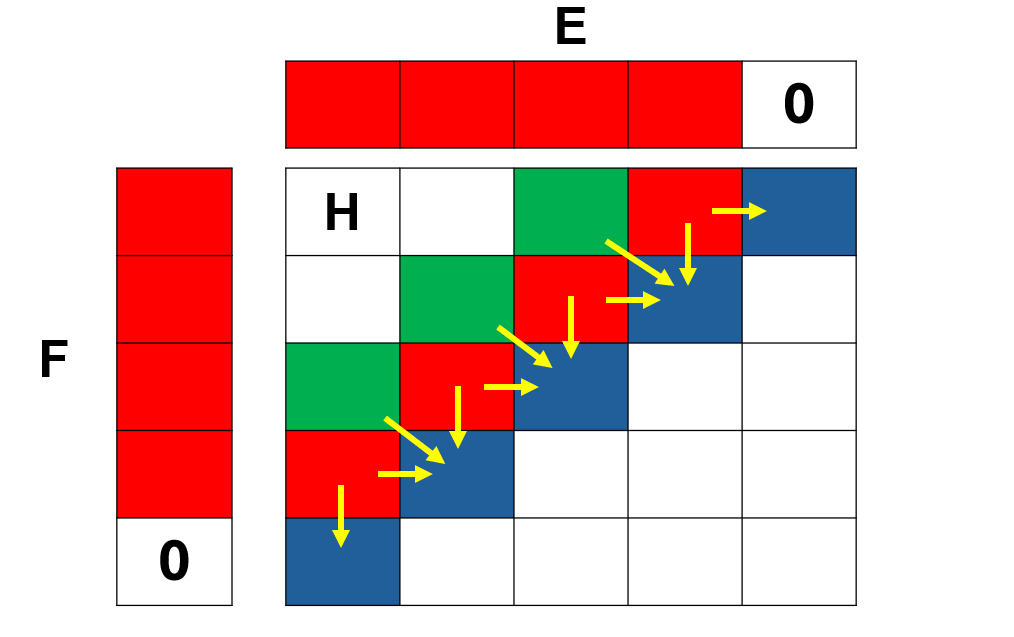
\includegraphics[width = 1\textwidth]{figures/Anti-Diagonal.png}
    \caption{Anti-Diagonal and Dependency diagram}
    \label{fig:Anti-Diagonal and Dependency diagram}
\end{figure}

\section{Coalesced Memory Access}
\textbf{Coalesced Memory Access}(Figure\ref{fig:Coalesced Memory Access}) is a technique in CUDA for optimizing global memory access efficiency. It primarily improves GPU performance by enhancing the utilization of global memory bandwidth. For example, when a warp (the number of threads that can actually execute simultaneously on the GPU at any one time, typically 32 or 64) accesses consecutive memory addresses in global memory, the memory requests from these threads can be grouped into a single large memory transaction. This significantly reduces the number of memory transactions and increases efficiency. In contrast, if the accessed addresses are not contiguous, each thread must initiate a separate memory transaction, resulting in a significant drop in access efficiency.

As mentioned at the end of the previous chapter, this study optimizes the memory layout of matrices $E$ and $F$ in \textbf{CUDAlign}~\cite{CUDAlign} by compressing the original two-dimensional matrices into one-dimensional arrays. This transformation converts the originally non-contiguous memory access pattern along the anti-diagonals into a contiguous access pattern in the arrays. This not only leverages the advantages of Coalesced Memory Access in CUDA but also increases the available memory space for matrix $H$ during a single GPU computation. Additionally, it reduces the number of context switches between the CPU and GPU, achieving a dual performance improvement.

\begin{figure}[ht]
    \centering
    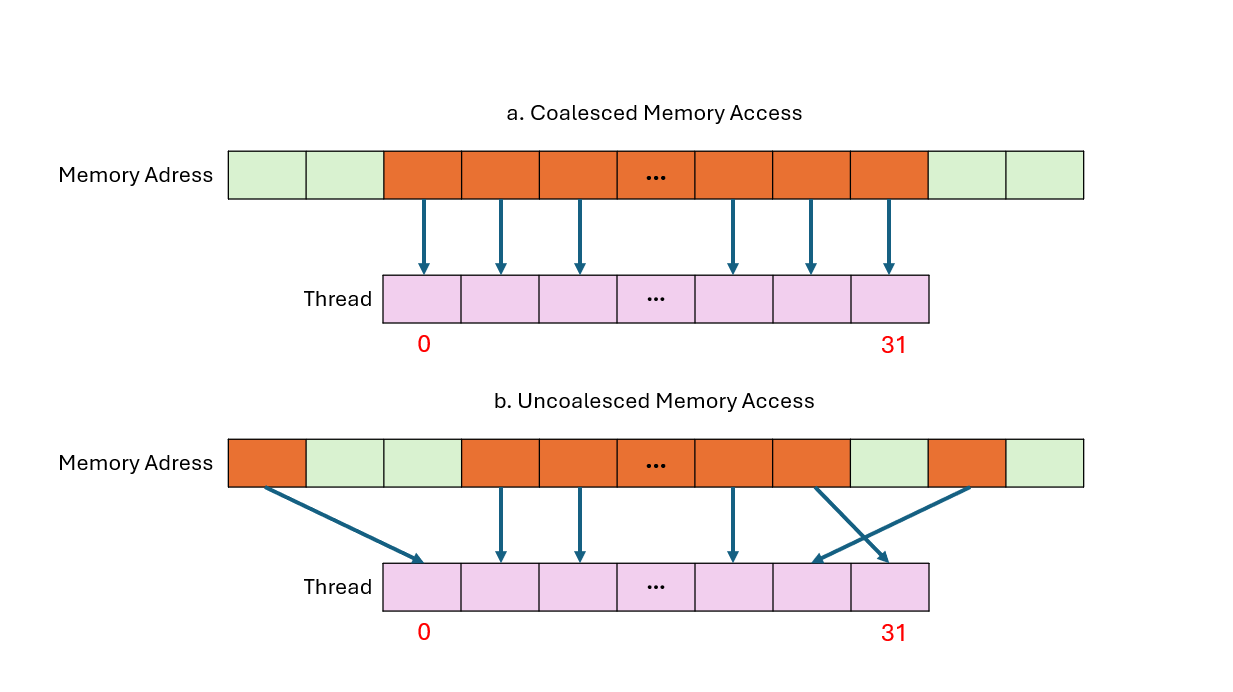
\includegraphics[width = 1\textwidth]{figures/Coalesced Memory Access.png}
    \caption{Coalesced Memory Access}
    \label{fig:Coalesced Memory Access}
\end{figure}

\section{Cell Delegation}
$Cell Delegation$ is an optimization technique applied within the anti-diagonal parallelization strategy, aimed at increasing the number of available threads per time step in the inner diagonal. Without the Cell Delegation technique, each block can initially activate only a single thread for computation. As the internal diagonals progress, it is not until the $T$-th diagonal (where $T$ is the number of threads assigned to each block) that full thread utilization and maximum parallelism is achieved. Starting from the $(T+1)$-th diagonal, the degree of parallelism gradually decreases again, eventually returning to a single active thread on the final diagonal. This causes a drop in execution performance.As illustrated in Figure~\ref{fig:Cells Delegation(Inner diagonal)}, the Cell Delegation technique redefines each block’s originally rectangular or square computation region into a parallelogram. All cells beyond the $T$-th inner diagonal are delegated to the blocks of the next outer diagonal, allowing those upcoming blocks to fully utilize all threads from the very first inner diagonal through to the last.

From the perspective of outer diagonals, this method significantly reduces the number of blocks suffering from low parallelism. Originally, all blocks encountered this issue. With Cell Delegation, only $\frac{n}{2T} + 1$ blocks remain affected, where $n$ is the sequence length in the horizontal direction, and $T$ is the number of threads assigned per block. The additional $+1$ accounts for the final outer diagonal, which lacks a subsequent diagonal to delegate to, thus requiring the creation of an extra diagonal to handle the remaining cells.

Figure~\ref{fig:Cells Delegation} shows the distribution of computation regions under the Cell Delegation strategy, as viewed from the perspective of outer diagonals.

\subsection{Data Harzard in Cell Delegation}
When implementing Cell Delegation in CUDA, there is a potential for data hazards to occur. This arises because, in a single CUDA kernel execution, the execution order of blocks is unpredictable—blocks can be executed either in parallel or sequentially. As shown in Figure \ref{fig:Cells Delegation}, blocks assigned along the same outer diagonal have overlapping regions in the vertical direction. Therefore, if a lower block is executed first or runs faster while the upper block has not yet completed computing the overlapping cells, a data hazard will occur during the lower block's computation.
To resolve this issue and ensure that blocks on the same outer diagonal compute under correct data dependencies, we must divide the computation of each outer diagonal into two separate kernel functions: the First Phase and the Second Phase. In the first phase, all blocks compute the first $T$ inner diagonals, then control is returned to the CPU, which launches the second-phase kernel to complete the remaining $n_B - T$ inner diagonals—ensuring the correct computation of a single outer diagonal. Here, $n_B$ is the length of the computation range assigned to each block, and $T$ is the width.Additionally, an extra condition must be satisfied: $n_B \ge 2T$. This requirement ensures that, due to the Cell Delegation technique, each inner diagonal in the next block can utilize full parallelism. Since the upper block leaves behind $T - 1$ columns of incomplete cells, the lower block can safely read up to $n_B - (T - 1)$ columns in the short phase without causing hazards. Therefore, in this study, we simply set $n_B = 2T$, which effectively eliminates the risk of data hazards.

\begin{figure}[htbp]
    \centering
    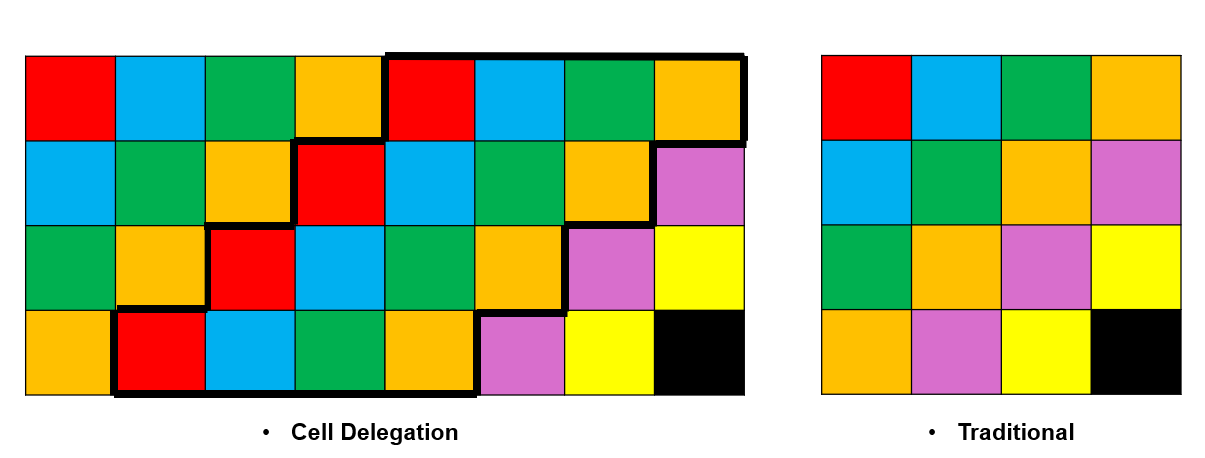
\includegraphics[height=6cm]{figures/Cell Delegation(Inner Block).png}
    \caption{Cells Delegation(Inner diagonal)}
    \label{fig:Cells Delegation(Inner diagonal)}
\end{figure}

\begin{figure}[htbp]
    \centering
    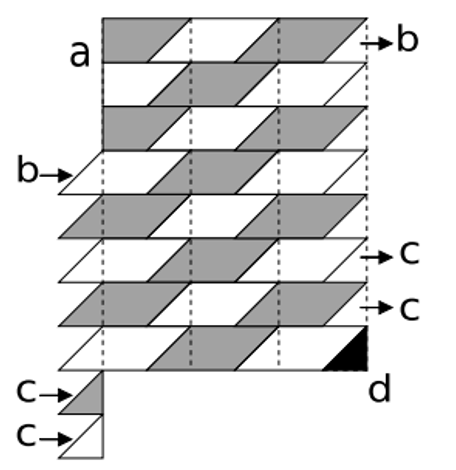
\includegraphics[height=8cm]{figures/Cell Delegation.png}
    \caption{Cells Delegation}
    \label{fig:Cells Delegation}
\end{figure}
\FloatBarrier
\section{Sliding Window}
In the Smith-Waterman algorithm with affine gap penalty, the space complexity is $O(mn)$, where $m$ and $n$ correspond to the mtDNA and nDNA in this study, respectively. Since the length of nDNA is approximately 3.2 billion base pairs, storing the entire matrix would require several tens of terabytes of memory. For a typical personal computer, not only is it impossible to hold such a large amount of memory, but even the storage capacity of the hard drive may be insufficient to handle such data volume. Moreover, Nvidia GPUs often come with memory limitations depending on the specific model. For instance, the GPUs used in this study, namely the \textbf{RTX 2070 SUPER} and \textbf{RTX 4080}, have memory capacities of 8GB and 16GB, respectively, which are far from sufficient to load the entire matrix into the GPU for accelerated computation.To address this, we adopt the \textbf{Sliding Window} strategy. Based on the current GPU memory limitation and the block assignment constraints described in the previous section, we calculate the maximum feasible length of nDNA segments that can be processed at one time. We then allocate and initialize the $H$ matrix and the $E$ and $F$ arrays on the GPU. After completing the computation for one window, we use dedicated kernel functions designed for data transfer and initialization to move the last column of data to the first column and reinitialize the values in the $E$ array, preparing them for the next window computation.

This approach not only leverages the GPU’s parallel computing capabilities to accelerate data transfer and initialization, but also enables the entire algorithm to be computed using a single set of matrices and arrays. As a result, it significantly reduces the data transfer overhead between the Host (CPU) and the Device (GPU). Figure \ref{fig:Sliding Window} illustrates the Sliding Window strategy.
\begin{figure}[htbp]
    \centering
    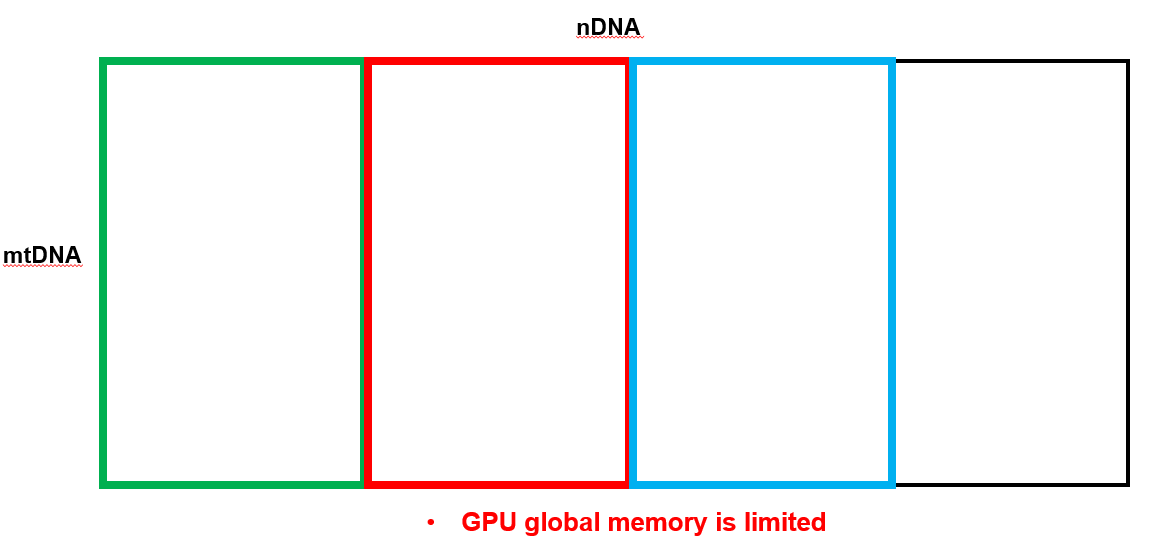
\includegraphics[width=1\linewidth]{figures/Sliding Window.png}
    \caption{Sliding Window Strategy}
    \label{fig:Sliding Window}
\end{figure}
\section{Workflow}
Figure\ref{fig:Workflow} illustrates the workflow between the Host and Device in this study. Starting from the Host side, the process can be divided into the following steps.
(1)\textbf{Data Initialization}: All required data is initialized on the Host (CPU), including scores and penalties, and the loading of mtDNA and nDNA sequences.
(2)\textbf{Data Slicing}: We calculate the maximum length of the nDNA segment that can be processed at a time. The $H$ matrix and the $E$ and $F$ arrays are then allocated and initialized accordingly.
(3)\textbf{Data Transfer from Host to Device}:The data prepared in the previous two steps is transferred from the Host (CPU) to the Device (GPU) memory to ensure the GPU has all the necessary data for computation.
(4)\textbf{Kernel Launch for every diagonal}:Based on the length of the $mtDNA$ and the configured number of threads and blocks, we calculate the number of outer diagonals. For each diagonal, a kernel function is launched to perform the algorithmic computations.
(5)\textbf{Data Movement and Data Transfer from Device to Host}:Once a round of matrix computation is completed, the data from the last column is moved to the first column to serve as input for the next computation window. Additionally, the maximum value of each column is transferred back to the Host for storage.
(6)\textbf{Repeat}:Steps (3) to (5) are repeated until the entire nDNA sequence has been fully aligned. At this point, we obtain the optimal alignment score and position, along with the maximum values and positions of each column. These results are saved to an output file for further visualization and analysis.
\begin{figure}[htbp]
    \centering
    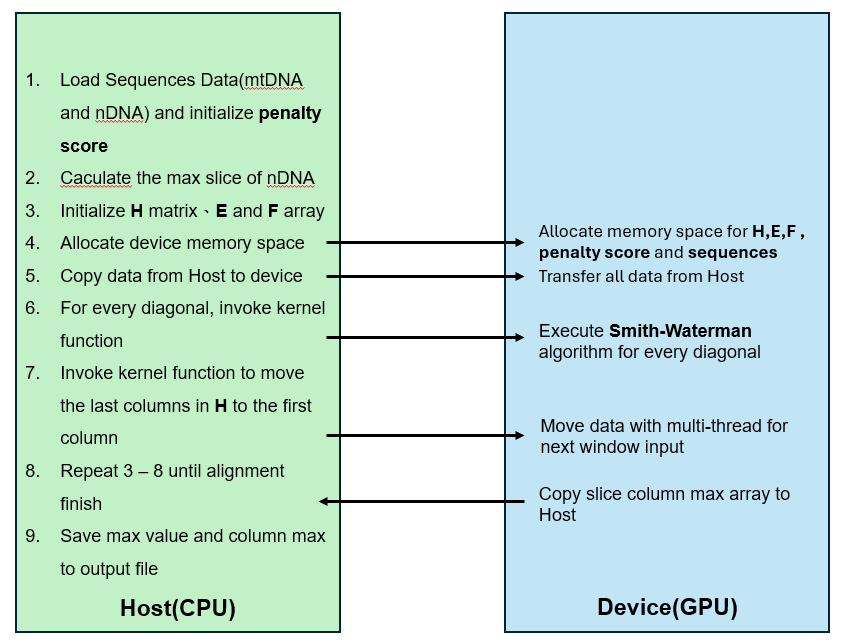
\includegraphics[width=1\linewidth]{figures/workflow.png}
    \caption{Workflow}
    \label{fig:Workflow}
\end{figure}

\subsection{Pseudo Code(Host)}

\begin{algorithm}
\caption{Pseudocode in Host(CPU)}
\begin{algorithmic}[1]
\Procedure{Process the Smith-Waterman with affine gap algorithm}{}
    \State Loading Sequences: $S_0= mtDNA$ and $S_1 = Chromesome_x$
    \State Set score and penalty and caculate max $sliceLen$ by $T$(threadsPerBlock) 
    \State Initialize Matrices and Arrays: $H_{0,j} = H_{i,0} = 0$, $F_i = 0$, $E_j = 0$
    \State Caculate total outer diagonal:$D$
    \For{$epoch = 0$ to $\frac{\text{len}(S_1)}{\text{sliceLen}}$}
        \State Transfer $S_1[epoch \times \text{sliceLen} : epoch \times \text{sliceLen} + \text{sliceLen}]$ to GPU
        \State Fill $E$ array with $0$
        \For{$k = 0$ to $D$}
            \State \texttt{First\_\_Phase} $<<< B, T>>>(D_k, H, E, F)$
            \State \texttt{Second\_\_Phase} $<<<B, T>>>(D_k, H, E, F)$
        \EndFor
        \State \texttt{Rest\_\_Row} $<<<1, T>>>(H, E, F)$
    \EndFor
    \State \textbf{Caculate the remaining columns}
    \State write $colmax$ array to the output file
    \State \textbf{return} max Score and its position 
\EndProcedure
\end{algorithmic}
\end{algorithm}

Algorithm 1 illustrates the procedure executed on the Host (CPU) side in this study. To compute the value of $sliceLen$ (i.e., the length of the chromosome segment that can be processed in each iteration), we base our calculation on the current GPU's maximum memory capacity, the length of the mtDNA, the number of configured threads, and the memory footprint of a single cell (32 bits). Additionally, there is a constraint that $sliceLen$ must be divisible by $2T$. The following inequality can be used to determine the maximum configurable segment length. From there, we simply find the largest value that satisfies the divisibility condition to determine the appropriate $sliceLen$.

\[
Global\_Memory\_Size \ge H\_Size + EF\_Size 
\]
\[
H\_Size = (\text{sliceLen} + 1)\times(\text{mtDNA\_Len} + 1) \times 32
\]
\[
EF\_Size = (\text{mtDNA\_Len} + \text{sliceLen}) \times 32
\]

Based on the obtained $sliceLen$, we can then calculate the values of $blocksPerGrid$ and the total number of outer diagonals using the following two formulas. With these, we can determine the total number of windows to compute and how many diagonals need to be processed in each iteration. Finally, we use a loop to invoke our kernel function accordingly.
\[
blocksPerGrid = \frac{sliceLen}{2\times threadsPerBlock}
\]
\[
totalOuterDiagonals = blocksPerGrid + \frac{mtDNA\_Len}{threadsPerBlock}
\]
At the end of the outer diagonal computation for each window, we additionally invoke a kernel function called $Rest_Row<<<1, T>>>$. This is because, in CUDAlign \cite{CUDAlign}, many of the formulas and calculations are based on the assumption that both $S_0$ and $S_1$ are divisible by $T$ and $B$. This assumption imposes a constraint on the number of usable threads—it must be a divisor of $S_0$. A more extreme case arises when the prime factorization of $S_0$ includes a very large prime number, which limits the GPU's ability to fully utilize its parallel processing power. To address this, we modified the program to allow users to specify the number of threads $T$. The portion of $S_0$ that is closest in length and divisible by $T$ is computed using the original parallel strategy. The remaining part (up to a maximum of $T-1$ rows) is then processed sequentially using one block along with cell delegation. This modification helps avoid such extreme scenarios and improves the flexibility of the program.

\subsection{Pseudo Code(Device)}
Algorithm 2 illustrates the \textbf{$First\_Phase$} kernel function that must be executed for each outer diagonal. The algorithm for \textbf{$Second\_Phase$} is similar, with the only differences being the initial value of $j$ and the fact that it does not require position checking or movement; the rest of the logic remains the same. Therefore, this paper focuses on explaining only the \textbf{$First\_Phase$}.

First, each thread calculates the position it needs to process using Algorithm 3. If $j < 1$, it indicates that the thread must handle the Cell Delegation part from the upper-right block of the previous round. Then, it checks whether the current position is within the valid region of the matrix. If it is valid, the computation is performed, and the value in the $colmax$ array is updated. After that, $\_\_syncthreads()$ is used to wait for all threads in the current inner diagonal to complete their computations and update the maximum score and its corresponding position. This process continues until all inner diagonals are processed.
\begin{algorithm}
\caption{GETCOORDINATE}
\begin{algorithmic}
\Procedure{}{}
    \State $block\_i = D_k - blockId;$
    \State $block\_j = blockId;$
    \State $i = (block\_i \times T) + threadId + 1$
    \State $block\_j \times C - threadId + 1$
\EndProcedure
\end{algorithmic}
\end{algorithm}
\begin{algorithm}
\caption{Kernel function in every Diagonal}
\begin{algorithmic}[1]
\Procedure{\textbf{$First\_Phase$}}{}
    \State \textbf{$i, j = GETCOORDINATE(D_k, blockId, threadId)$}
    \If{$j < 1$}
        \State i = i - $B$\times$T$
        \State j = $sliceLen$ + j
    \EndIf
    \For{$inner = 0$ to $T$}
        \If{$i \ge 1$ and $i \leq (mtDNA\_Len / T)\times T$  and $j <= restLen$}
            \State Caculate $H$, $E$ and $F$ cell value
            \State Update column max array
            \State Store cell value into sharedMemory
        \EndIf
        \State j++
        \If{$j == sliceLen + 1$}
            \State i = i + $B$\times$T$
            \State j = 1
        \EndIf
        \State $\_\_syncthreads()$
        \State Update maxScore and position with atomic
        \State $\_\_syncthreads()$
    \EndFor
\EndProcedure
\end{algorithmic}
\end{algorithm}

\chapter{Results}
\section{Data}
In this study, we selected the human mitochondrial DNA ($NC_012920.1$) from the \textbf{NCBI RefSeq} database as the reference sequence for mitochondrial analysis. The mtDNA has a total length of 16,806 bases. For the nuclear DNA (nDNA), we used the human whole genome from the \textbf{Ensembl GRCh38} release and specifically chose chromosomes 1 and 2 as the targets for our experiments. This selection was primarily aimed at accelerating the experimental process. Running a Smith-Waterman alignment with affine gap on a CPU between the mitochondrial genome and a single chromosome takes approximately one day. If we were to perform the alignment against the entire human genome, it could take nearly a month. Therefore, we selected a single chromosome as the nuclear genome target for mitochondrial comparison in this experiment.
\section{Experiment Setup}
The experimental setup in this study consists of two desktop computers. The primary system is equipped with an Intel Core i7-11700 processor featuring 8 cores, 16 threads, and a base clock speed of 2.5 GHz, along with an NVIDIA GeForce RTX 2070 GPU. To ensure the portability and general applicability of the proposed method, we also conducted experiments on a separate desktop equipped with an NVIDIA GeForce RTX 4080 GPU.Additionally, all experiments in this study were conducted using the same set of scoring and penalty parameters: \textbf{Match = 2}, \textbf{Mismatch = -3}, \textbf{OpenGap = -5}, and \textbf{ExtendGap = -2}.

\section{Benchmark}
To evaluate the performance of our proposed GPU-accelerated method, we used a single-core CPU implementation of the Smith-Waterman algorithm with affine gap penalties to perform alignments between the mtDNA and chromosomes, serving as the benchmark for this study. Due to the limited memory capacity of the CPU, which is insufficient to hold the entire scoring matrix, the CPU-based computation was also carried out using a sliding window approach.

\section{Configuration setting}
Before comparing the performance differences and speedup between the method proposed in this study and the benchmark, we must first determine the optimal number of $threadPerBlock$ settings for different GPUs to achieve the best performance. To this end, we tested four different $threadPerBlock$ configurations: 32, 64, 96, and 128. These values were chosen as they are multiples of 32, which corresponds to the typical warp size (32 or 64 threads) in NVIDIA GPUs.
Tables \ref{tab:20701} \ref{tab:20702} \ref{tab:40801} \ref{tab:40802} present the execution times of \textbf{NVIDIA GeForce RTX 2070} and \textbf{NVIDIA GeForce RTX 4080}, respectively, under different threadPerBlock configurations for comparing different chromosomes. The results show that the optimal performance on the \textbf{NVIDIA GeForce RTX 2070} is achieved with 64 threads, while on the \textbf{NVIDIA GeForce RTX 4080}, the best performance is obtained with 96 threads. Therefore, in the subsequent performance comparisons and speedup charts, we use these optimal configurations for comparison against the benchmark.

\begin{table}[h]
    \centering
    \caption{RTX 2070 Super Comparison in Chromosome1}
    \label{tab:20701}
    \begin{tabular}{|c|c|c|c|c|c|c|}
        \hline
         \textbf{Device} & \textbf{mtDNA\_len}& \textbf{nDNA\_len}& \textbf{Threads} & \textbf{Blocks} & \textbf{Time (Sec)} & \textbf{Convert Time} \\
        \hline
         2070 SUPER & 16806 & 253095529 & 32 & 237 & 2310 & 38 mins \\
        \hline
         \rowcolor{yellow}
         2070 SUPER & 16806 & 253095529 & \textbf{64} & 118 & 2091 & 35 mins \\
        \hline
         2070 SUPER & 16806 & 253095529 & 96 & 79 & 2418 & 40 mins \\
        \hline
         2070 SUPER & 16806 & 253095529 & 128 & 59 & 2887 & 48 mins \\
         \hline
    \end{tabular}
\end{table}

\begin{table}[h]
    \centering
    \caption{RTX 2070 Super Comparison in Chromosome2}
    \label{tab:20702}
    \begin{tabular}{|c|c|c|c|c|c|c|}
        \hline
         \textbf{Device} & \textbf{mtDNA\_len}& \textbf{nDNA\_len}& \textbf{Threads} & \textbf{Blocks} & \textbf{Time (Sec)} & \textbf{Convert Time} \\
        \hline
         2070 SUPER & 16806 & 246219922 & 32 & 237 & 2326 & 38 mins \\
        \hline
         \rowcolor{yellow}
         2070 SUPER & 16806 & 246219922 & \textbf{64} & 118 & 2043 & 34 mins \\
        \hline
         2070 SUPER & 16806 & 246219922 & 96 & 79 & 2432 & 40 mins \\
        \hline
         2070 SUPER & 16806 & 246219922 & 128 & 59 & 3061 & 51 mins \\
         \hline
    \end{tabular}
\end{table}

\begin{table}[h]
    \centering
    \caption{RTX 4080 Comparison in Chromosome1}
    \label{tab:40801}
    \begin{tabular}{|c|c|c|c|c|c|c|}
        \hline
         \textbf{Device} & \textbf{mtDNA\_len}& \textbf{nDNA\_len}& \textbf{Threads} & \textbf{Blocks} & \textbf{Time (Sec)} & \textbf{Convert Time} \\
        \hline
         RTX 4080 & 16806 & 253095529 & 32 & 489 & 1120 & 19 mins \\
        \hline
         RTX 4080 & 16806 & 253095529 & 64 & 244 & 1115 & 19 mins \\
        \hline
         \rowcolor{yellow}
         RTX 4080 & 16806 & 253095529 & \textbf{96} & 163 & 1059 & 18 mins \\
        \hline
         RTX 4080 & 16806 & 253095529 & 128 & 122 & 1352 & 23 mins \\
         \hline
    \end{tabular}
\end{table}

\begin{table}[h]
    \centering
    \caption{RTX 4080 Comparison in Chromosome2}
    \label{tab:40802}
    \begin{tabular}{|c|c|c|c|c|c|c|}
        \hline
         \textbf{Device} & \textbf{mtDNA\_len}& \textbf{nDNA\_len}& \textbf{Threads} & \textbf{Blocks} & \textbf{Time (Sec)} & \textbf{Convert Time} \\
        \hline
         RTX 4080 & 16806 & 246219922 & 32 & 489 & 1090 & 18 mins \\
        \hline
         RTX 4080 & 16806 & 246219922 & 64 & 244 & 1080 & 18 mins \\
        \hline
         \rowcolor{yellow}
         RTX 4080 & 16806 & 246219922 & \textbf{96} & 163 & 1024 & 17 mins \\
        \hline
         RTX 4080 & 16806 & 246219922 & 128 & 122 & 1313 & 22 mins \\
         \hline
    \end{tabular}
\end{table}

\clearpage
\subsection{Speedup}
Tables \ref{tab:result1} \ref{tab:result2} and Figures \ref{fig:result1} \ref{fig:result2} respectively show the comparison of execution time and SpeedUp between two Nvidia GPU devices and the benchmark (CPU version). It is evident that the CUDA method developed in this study demonstrates strong performance both in terms of actual execution time and Speedup. On the \textbf{RTX 2070 SUPER}, a Speedup of over 30× can be achieved, while execution on the \textbf{RTX 4080} is twice as fast as on the \textbf{RTX 2070 SUPER}. Originally, the CPU version required nearly a full day to complete the computation, but with our method, the process can be finished in approximately 20 minutes. This suggests that as GPU hardware continues to advance and computing power increases, our method holds great potential for achieving even faster performance in the future.

\begin{table}[h]
    \centering
    \caption{Result (Chromosome1)}
    \label{tab:result1}
    \begin{tabular}{|c|c|c|c|}
     \hline
      \textbf{Device} & \textbf{Time (Sec)} &\textbf{Speedup} & \textbf{Convert Time} \\
     \hline
      CPU & 78439 & 1 & 22 hours\\
     \hline
      2070 & 2091 & \textbf{37.51} & 35 mins\\
     \hline
      4080 & 1059 & \textbf{74.06} & 18 mins\\
     \hline
    \end{tabular}
\end{table}

\begin{figure}[htbp]
    \centering
    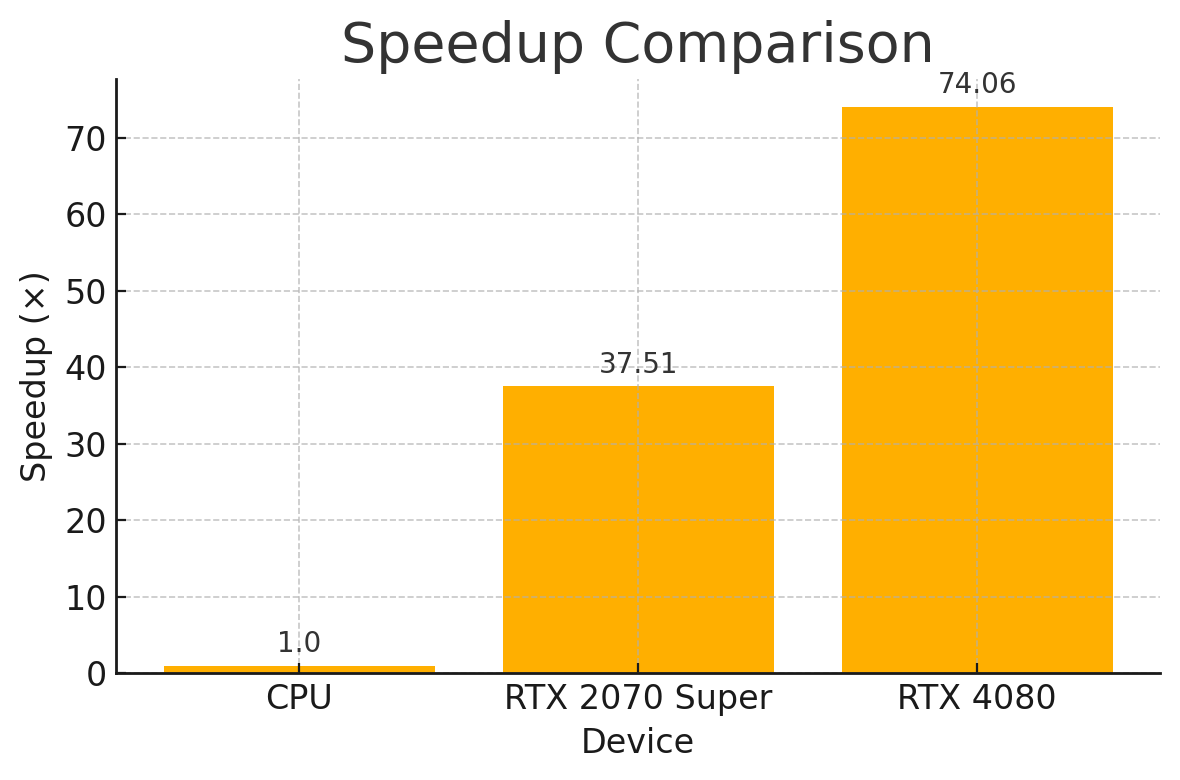
\includegraphics[height=8cm]{figures/Result1.png}
    \caption{Sppedup(Chromosome1)}
    \label{fig:result1}
\end{figure}

\begin{table}[h]
    \centering
    \caption{Result(Chromosome2)}
    \label{tab:result2}
    \begin{tabular}{|c|c|c|c|}
     \hline
      \textbf{Device} & \textbf{Time (Sec)} &\textbf{Speedup} & \textbf{Convert Time} \\
     \hline
      CPU & 72444 & 1 & 20 hours\\
     \hline
      2070 & 2043 & \textbf{35.46} & 34 mins\\
     \hline
      4080 & 1024 & \textbf{70.75} & 17 mins\\
     \hline
    \end{tabular}
\end{table}

\begin{figure}[htbp]
    \centering
    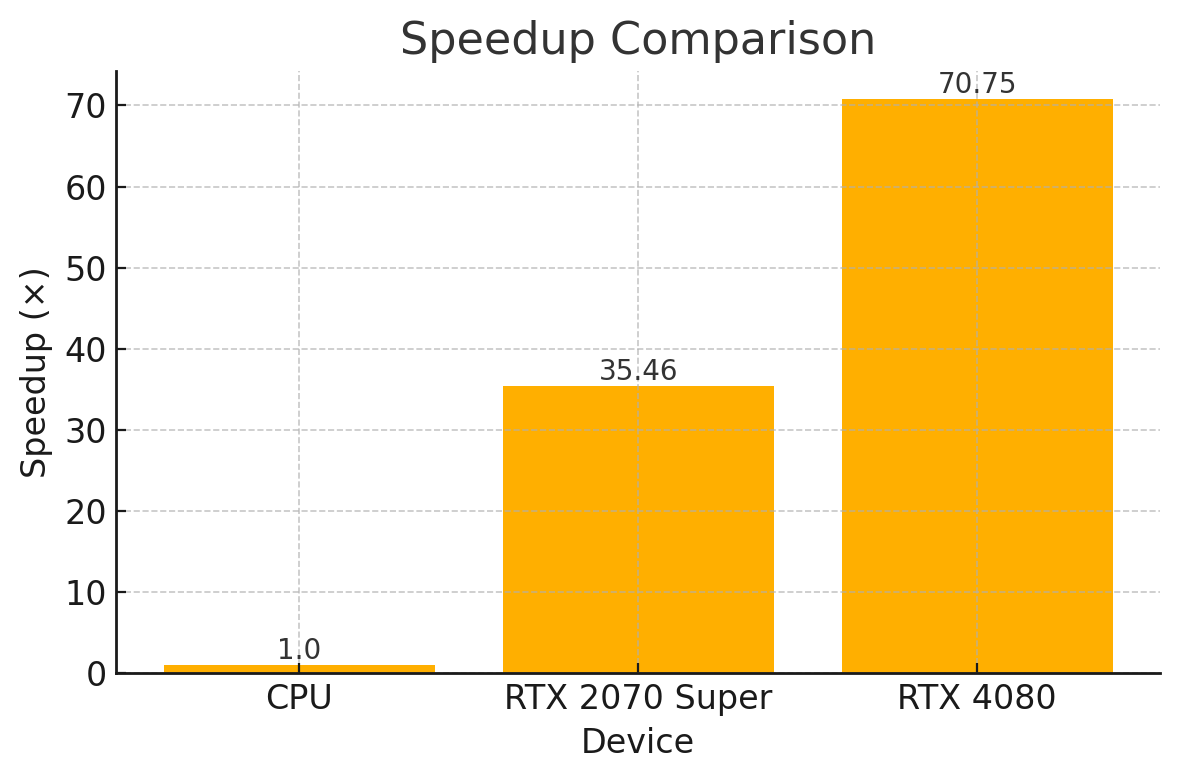
\includegraphics[height=8cm]{figures/Result2.png}
    \caption{Sppedup (Chromosome2)}
    \label{fig:result2}
\end{figure}
\subsection{Segments}
The ultimate goal of performing local alignment with an affine gap algorithm is to identify highly similar regions between sequences. Due to memory limitations mentioned earlier, we are unable to store the entire alignment matrix. Therefore, we utilize an array with a length equal to that of the nDNA (chromosome) to store the maximum score and its corresponding position for each column. The stored information includes $i$, $j$, and the alignment $score$. This data is then saved to a file.To determine whether the maximum values in each column lie on the same traceback path or are located in nearby regions, we first set a threshold to filter out positions with scores below this value. Next, based on the score penalty and another user-defined parameter called $step$, we assess whether two adjacent points can be connected. If they can be connected, they are considered part of the same segment.
\\
\begin{figure}[htbp]
    \centering
    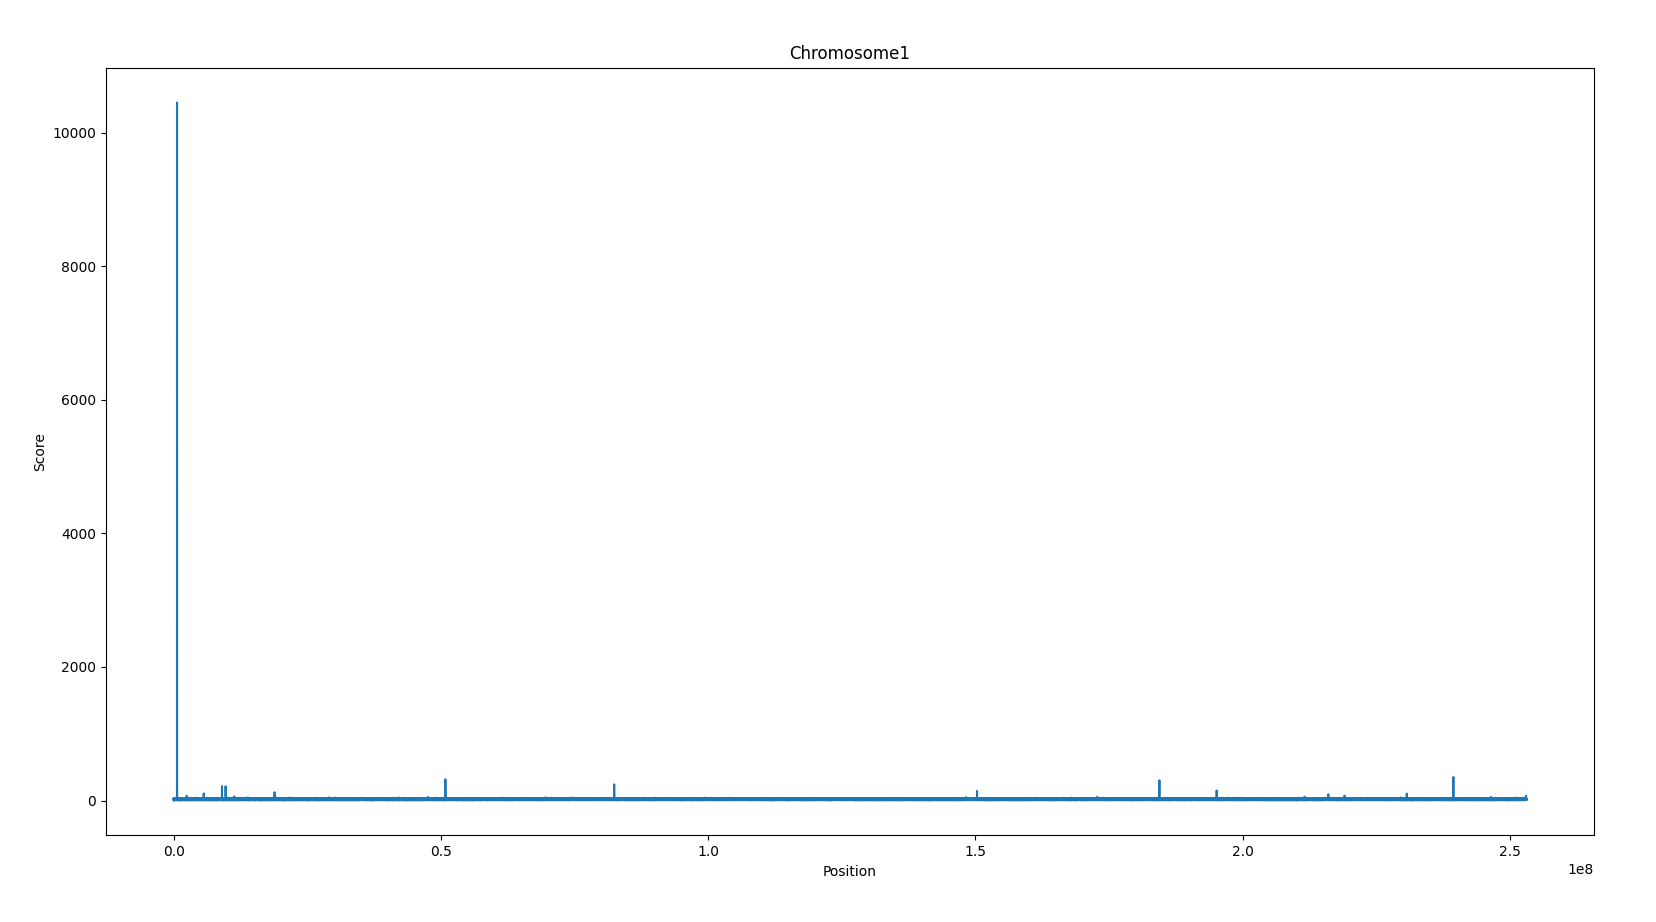
\includegraphics[width=1\linewidth]{figures/chromosome1Distribution.png}
    \caption{Chromosome1(Column Max Distribution)}
    \label{fig:chromosome1Distribution}
\end{figure}

\begin{figure}[htbp]
    \centering
    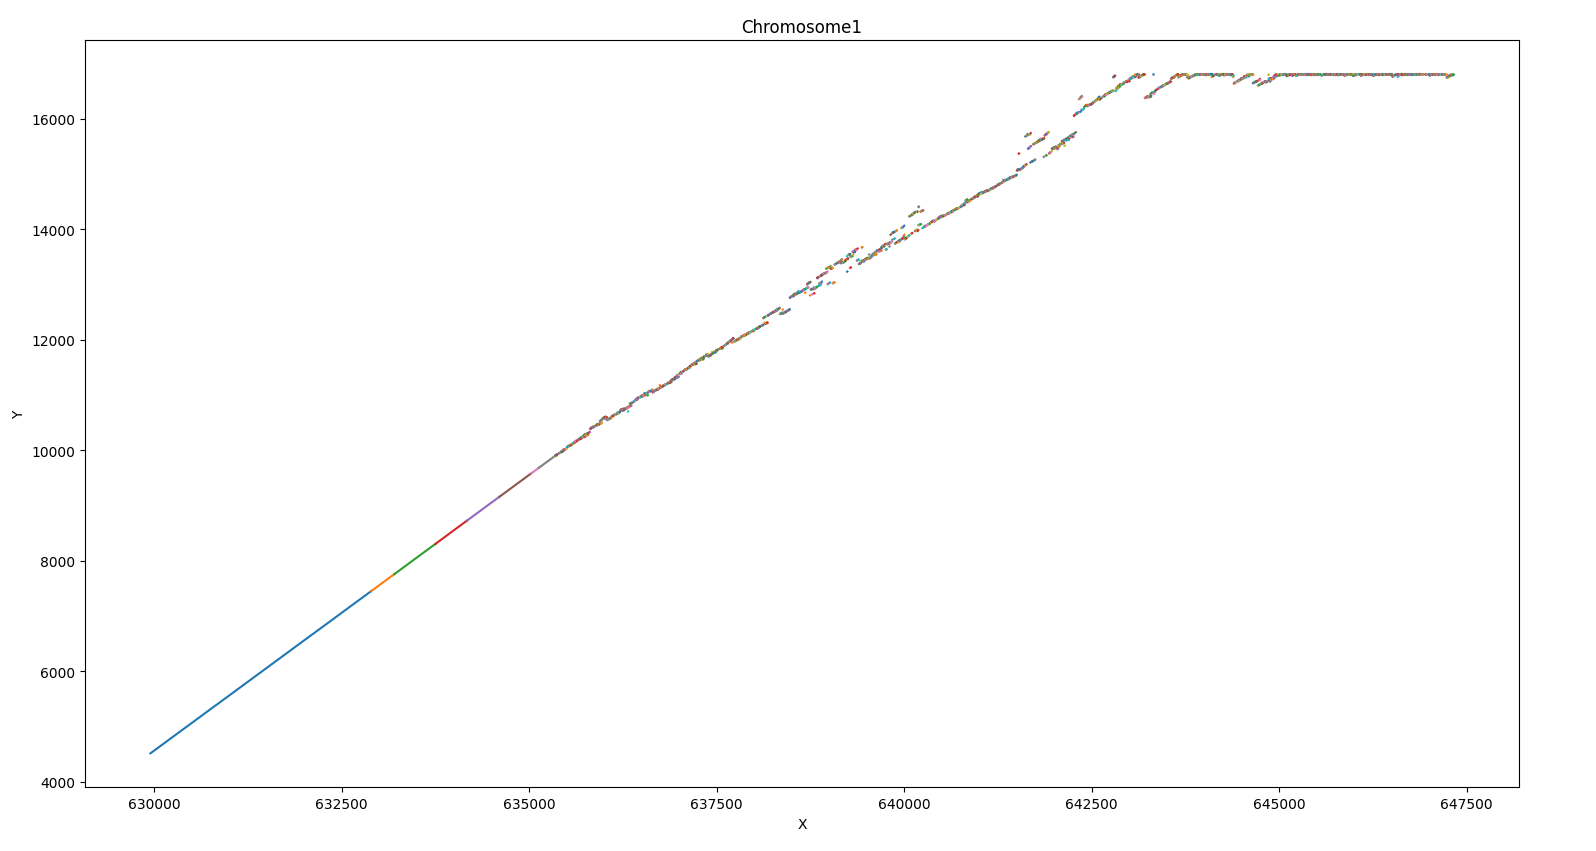
\includegraphics[width=1\linewidth]{figures/chromosome1threshold 1000.png}
    \caption{Chromosome1(threshold = 1000)}
    \label{fig:chromosome1threshold1000}
\end{figure}

\begin{figure}[htbp]
    \centering
    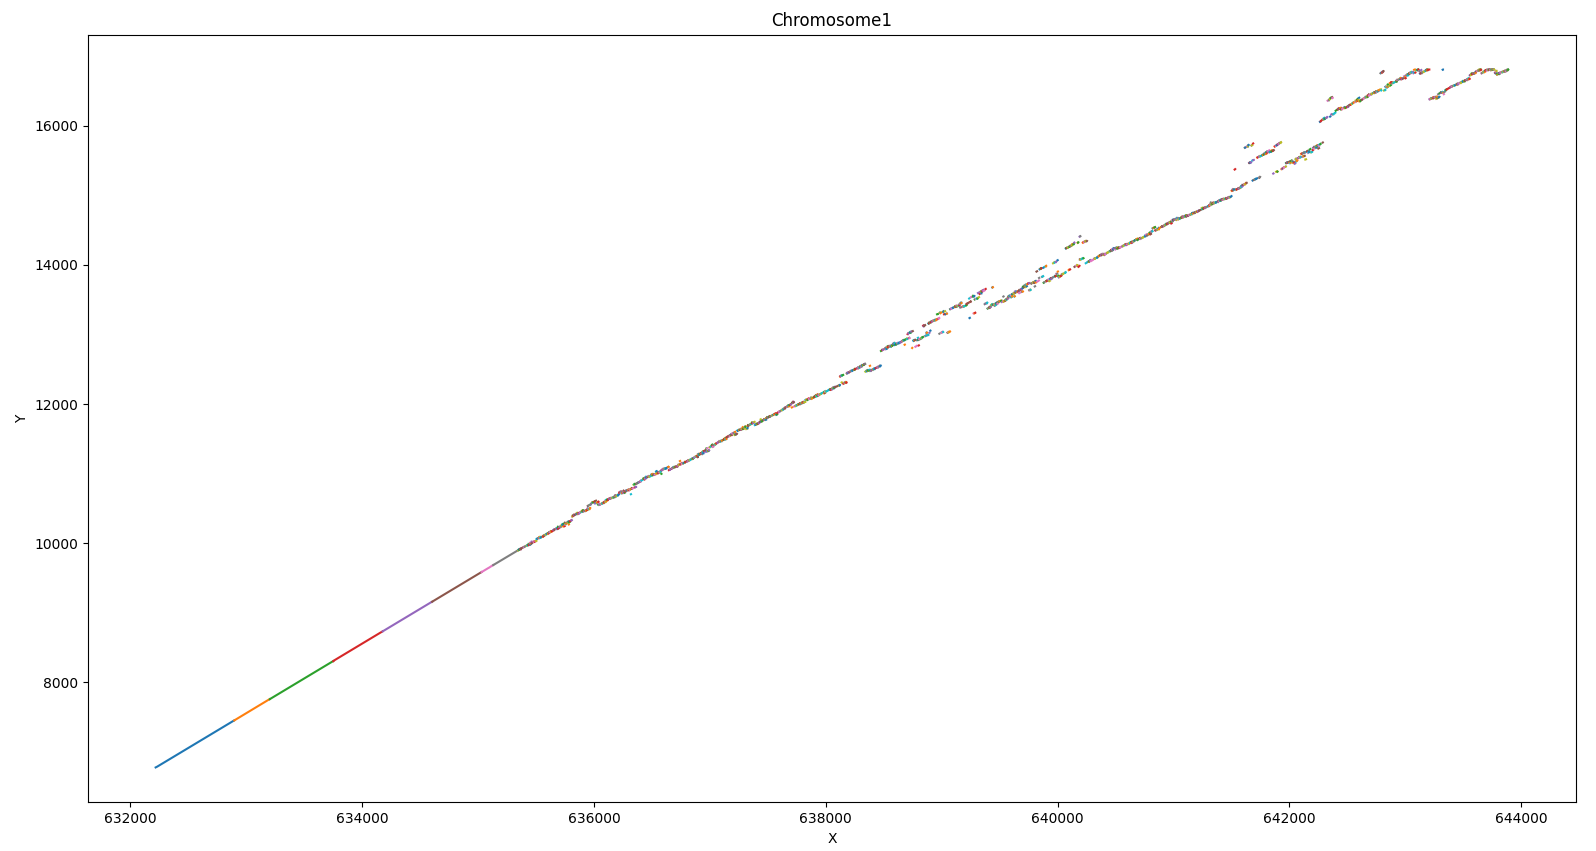
\includegraphics[width=1\linewidth]{figures/chromosome1threshold 5000.png}
    \caption{Chromosome1(threshold = 5000)}
    \label{fig:chromosome1threshold5000}
\end{figure}

Figure \ref{fig:chromosome1Distribution} shows the score distribution of the maximum values at each horizontal position when aligning mtDNA to chromosome 1. Due to the considerable length of the chromosome, compressing the score display space causes many non-zero scores to appear as zeros. Subsequently, Figures \ref{fig:chromosome1threshold1000} and \ref{fig:chromosome1threshold5000} illustrate the segment identification results using a $threshold$ of 1000 and 5000, respectively, with a fixed $step$ of 10. We can observe that the qualified positions are clustered within the same region, allowing us to infer that the algorithm successfully identifies the local regions where the $chromosome$ and $mtDNA$ are similar.

\begin{figure}[htbp]
    \centering
    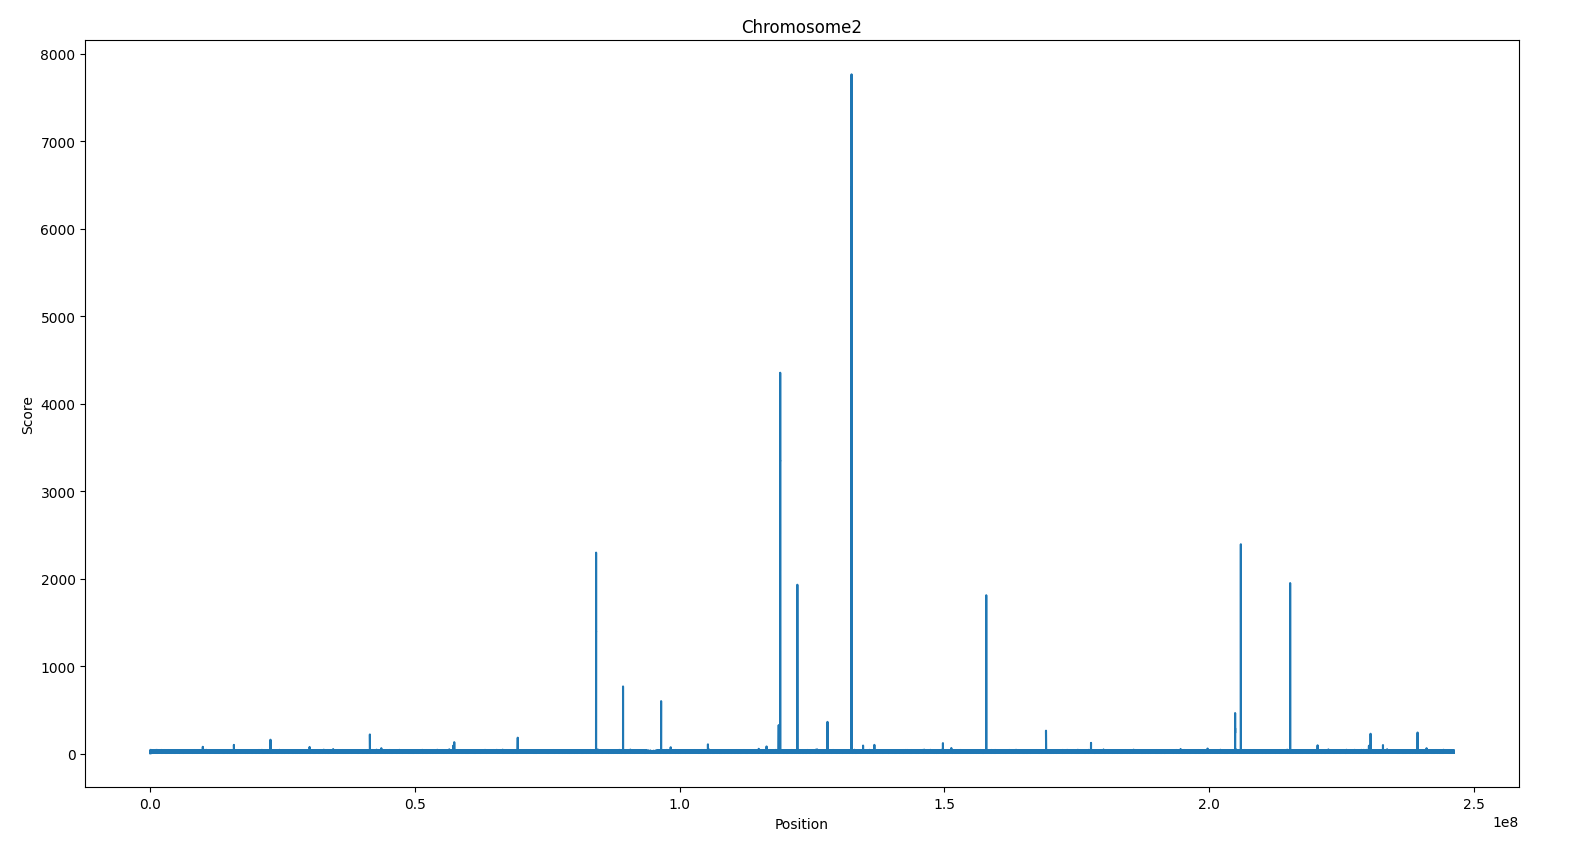
\includegraphics[width=1\linewidth]{figures/chromosome2Distribution.png}
    \caption{Chromosome2(Column Max Distribution)}
    \label{fig:chromosome2Distribution}
\end{figure}

\begin{figure}[htbp]
    \centering
    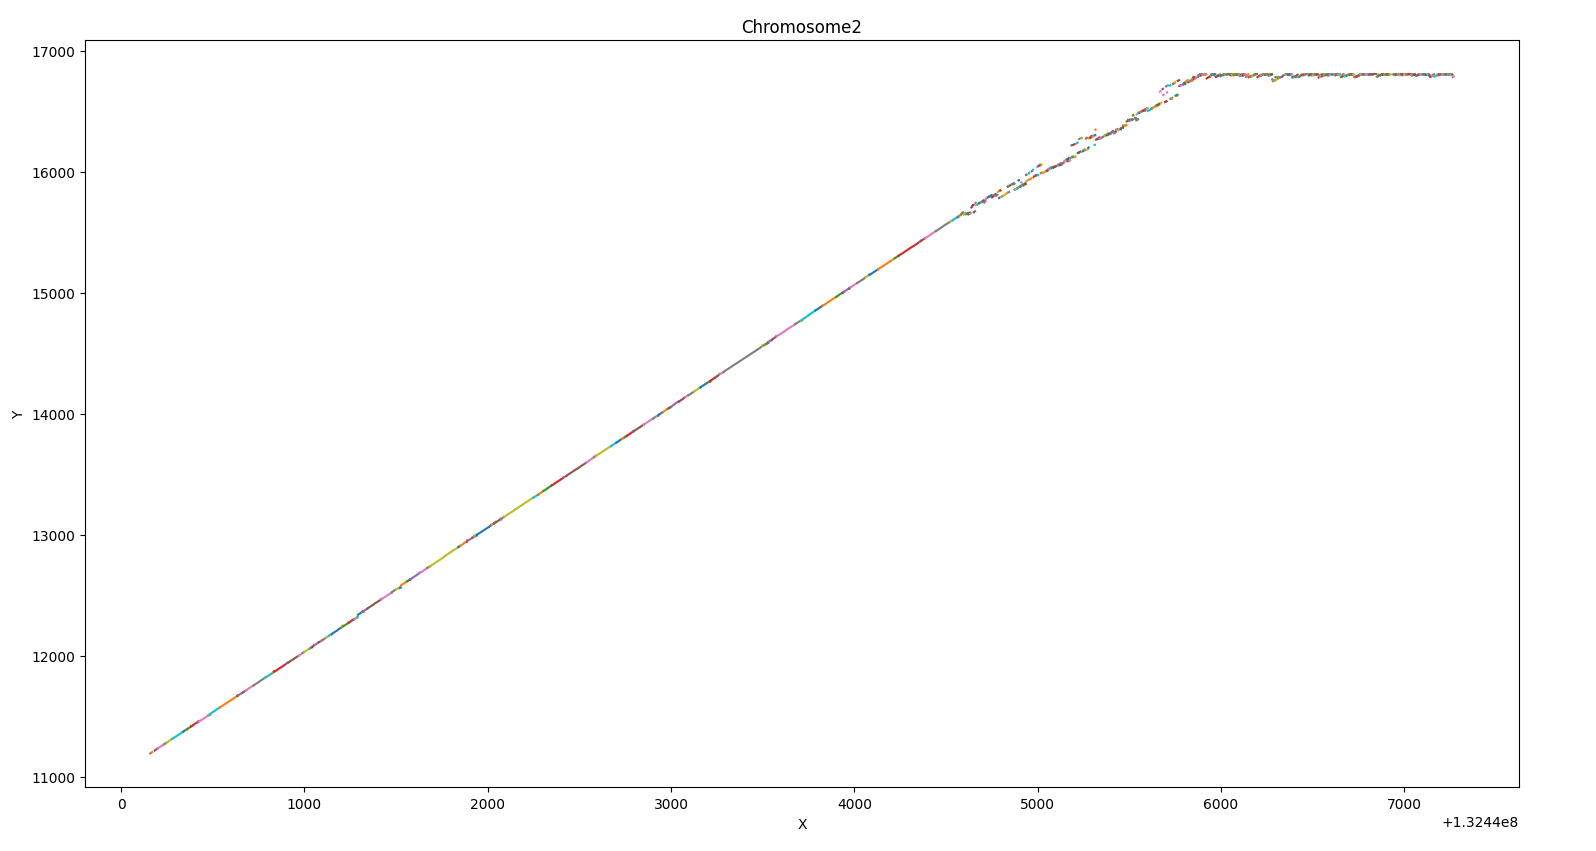
\includegraphics[width=1\linewidth]{figures/chromosome2threshold5000.png}
    \caption{Chromosome2(threshold = 5000)}
    \label{fig:chromosome2threshold5000}
\end{figure}

Figure \ref{fig:chromosome2Distribution} shows the score distribution of the maximum values at each horizontal position when aligning mtDNA to chromosome 2, while Figure \ref{fig:chromosome2threshold5000} illustrates the local alignment segments identified under the conditions of $threshold=5000$ and $step = 10$. Using this method, analysts can set their own score thresholds of interest to examine the alignment results and corresponding positions.

\chapter{Discussion}
Based on the results of this study, the GPU-accelerated implementation of the Smith-Waterman algorithm with affine gap penalty demonstrates significant performance improvements in the alignment tasks between mitochondrial DNA (mtDNA) and chromosomal sequences. This showcases the advantages of GPU parallel processing. In the comparison between mtDNA and Chromosome 1, we achieved speedups of 37.51 and 74.06 on the RTX 2070 SUPER and RTX 4080, respectively. For Chromosome 2, the speedups were 35.46 and 70.75, respectively. These results far exceeded our initial expectations.From a practical standpoint, the traditional method would take more than 20 hours to complete a single alignment task. In contrast, our GPU-accelerated approach reduces this time to just 30 minutes, and with a higher-end device like the RTX 4080, the runtime can be further reduced to approximately 17 minutes. This not only highlights the direct impact of hardware upgrades on computational performance but also confirms the scalability of our proposed method.

To ensure the practical usability and reproducibility of our tool, we used datasets sourced from publicly available bioinformatics databases. For researchers performing full human genome alignments (across all 23 chromosomes), the conventional approach may take at least 20 days to complete. However, with our developed tool, the same task can be completed in just around 7 hours, significantly accelerating research timelines.Additionally, we have integrated a graphical user interface that allows users to quickly visualize alignment regions of interest based on their specific needs. While the speedup figures demonstrate numerical improvements, the real value of our method lies in the enhanced flexibility and usability it offers. Furthermore, the approach we propose is not limited to mtDNA and nuclear DNA (nDNA) alignment; it is also applicable to any large-scale genome sequence alignment where there is a considerable difference in sequence length, thus broadening its range of applications.We believe that as GPU hardware technology continues to advance, our method will be capable of delivering even greater computational power, ushering in a transformative leap in biological sequence analysis.

\section{Future Work}
There are some future improvements we can try.\\
(1) Sequence Compression: In this study, each sequence segment (window) to be aligned is stored in read-only constant memory to accelerate memory access during alignment. However, constant memory has limited capacity. If the usable global memory increases in the future—allowing longer sequences to be aligned—constant memory might become insufficient. One possible solution is sequence compression. Since each base in DNA consists of only five possible characters: A, C, G, T, and N, we can compress each character from the original 8 bits to 4 bits. This allows more sequence data to fit within the fixed capacity of constant memory, effectively extending the length of sequences that can be stored. Additionally, this compression can reduce the frequency of CPU-GPU context switches, improving overall performance.

(2) GPU Cluster: In this study, we focused solely on performance optimization using a single GPU and did not explore parallel processing of multiple sequence alignments. In the future, we could employ distributed computing or install multiple GPUs on a single machine to build a GPU computing cluster. This would enable our algorithm to run simultaneously across multiple GPUs, achieving a higher degree of parallelism and significantly improving performance and efficiency. For instance, based on the experiments in this study, if we could align different chromosomes in parallel across 23 GPUs, we could complete the alignment of the entire human genome in as little as half an hour.

\chapter{Conclusion}
In this study, we implemented a Smith-Waterman algorithm with affine gap penalties tailored for aligning genomic sequences of vastly different lengths. The implementation leverages anti-diagonal parallelization, cell delegation, compressed memory usage for improved coalesced memory access, and optimizes utilization of various memory hierarchies in CUDA architecture to accelerate GPU access efficiency. Additionally, we provide a visualization tool to facilitate analysis and ensure the portability of the program.

This tool not only offers significant convenience for researchers working on sequence alignment but also serves as a valuable reference framework for others in the field. Researchers can customize and extend the tool by adjusting parameters such as $Match$, $Mismatch$, $openGap$, and $extendGap$, or by modifying the core computation to switch from local to global alignment, enabling more tailored and advanced research applications.



\newpage
\AddToContents{Bibliography}
\printbibliography


\end{document}
